\section{ULF Parsing}

\begin{figure}
\centering
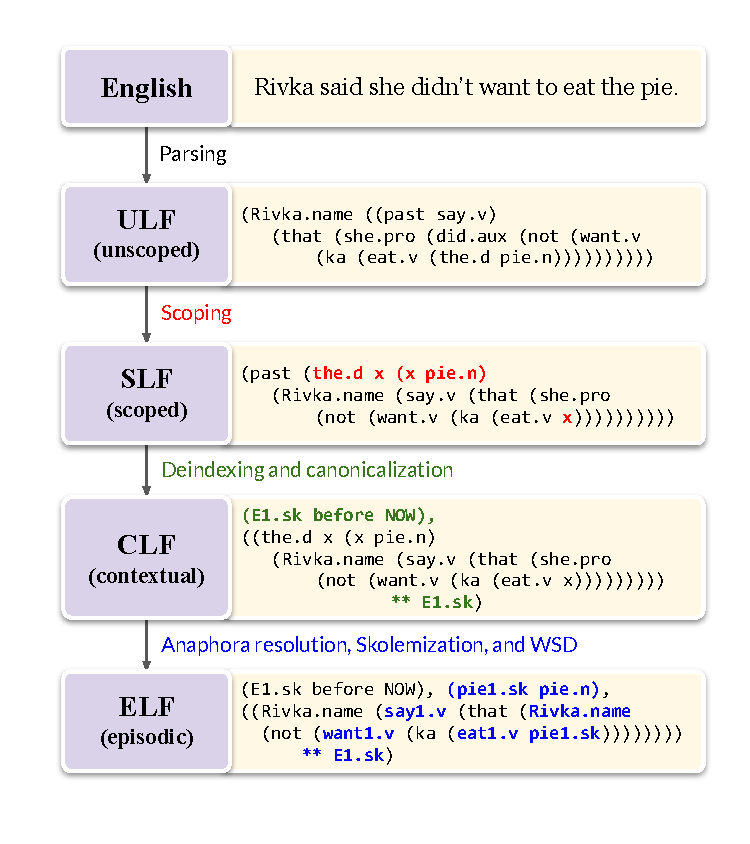
\includegraphics[width=\columnwidth]{CH2_el/el_pipeline.pdf}
\label{fig:el_pipeline}
\caption{The stages of the Episodic Logic parsing pipeline. Solid arrows represent the flow of data through the pipeline, and are labeled with the steps needed to obtain the target forms. The relevant changes are highlighted in each stage's example.}
\end{figure}

\label{subsec:ulf}
Unscoped Logical Form (ULF), an intermediate form of Episodic Logic, formally represents the semantic types and predicate-argument structures of natural language. It is the first, and most developed, step in the ``divide and conquer'' approach to EL parsing illustrated in Figure~\ref{fig:el_pipeline}. In order to obtain ELFs from ULFs, one must, at the very least, perform quantifier scoping, resolve anaphora, deindex the temporal coordinates of events, and disambiguate word senses, and \textit{canonicalization} (the minimization of ELFs into separate propositions by Skolemizing existentially quantified variables at the top level).

\citet{kim2022corpus} fully describes ULF and the current state of ULF parsing. In this section, we describe our language model-based ULF parser \citep{gibson2022language} and evaluate it against two other ULF parsers: a symbolic, rule-based transduction from constituency parses \citep{kim2021naloma} and a neural cache transition parser \citep{kim2021transition}, ultimately justifying our choice of the rule-based transduction method.

\subsection{Language Model-Based ULF Parsing}
In crafting an EL parsing pipeline, we experimented with using GPT-2, a state-of-the-art language model architecture based on a decoder-only transformer \citep{Radford2019LanguageMA}. Our intuition was that, given ULF's similarity to the syntactic surface form of English, a pre-trained language model might be able to perform well at ULF parsing by casting the problem as one of translation. In this light, we fine-tuned GPT-2 models to perform translation not just of English into ULF (parsing), but of ULF into English (verbalization). This section describes those models and the experiments performed on them.
\subsubsection{Objective}
%Like \citet{gpt-too}, we chose to fine-tune the GPT-2 \citep{Radford2019LanguageMA} language model to perform both of our tasks. Our approach differs slightly in that we did not adapt the default tokenizer to the ULF syntax, nor did we add the \texttt{\textbf{<SEP>}} or \texttt{\textbf{<END>}} tokens to the GPT-2 vocabulary, as modifying the tokenizer did not meaningfully improve performance on either task.
Given a tokenized English sentence $e = e_{1} \cdot e_{2} \cdot \ldots \cdot e_{m}$ and a tokenized s-expression representation of a corresponding ULF $u = u_{1} \cdot u_{2} \cdot \ldots \cdot u_{n}$, we fine-tuned our English-to-ULF GPT2 model for 327 epochs to maximize the joint probability of the concatenated sequences \footnote{The special tokens \texttt{<SEP>} and \texttt{<END>} were included between and after the two concatenated sequences, respectively, for every pair in the dataset.} $e$ and $u$, $P_{\textrm{GPT2}}(u,e) = P_{\textrm{GPT2}}(u|e) \cdot P_{\textrm{GPT2}}(e)$, where:

\vspace{3mm}

$$\mathlarger{P_{\textrm{GPT2}}(u|e) = \prod_{i=1}^{n} P_{\textrm{GPT2}}(u_{i} | e_{1:m},u_{1:i-1})}$$
\vspace{1mm}

$$\mathlarger{P_{\textrm{GPT2}}(e) = \prod_{j=1}^{m} P_{\textrm{GPT2}}(e_{j} | e_{1:j-1})}$$

\vspace{3mm}

The maximization objective for the ULF-to-English verbalization model is obtained by instead decomposing the joint probability $P_{\textrm{GPT2}}(u,e)$ into the similarly defined $P_{\textrm{GPT2}}(e|u)$ and $P_{\textrm{GPT2}}(u)$.

\subsubsection{Dataset}

We used the hand-annotated ULF dataset provided by \citet{kim2021transition}, comprising 1,738 sentences. We split our training (1,378), development (180), and test (180) sentences as prescribed in that paper. The data splitting aims to evenly distribute document-level topics among each subset of the sentences, and to avoid score inflation from linguistic similarity between adjacent sentences.

%For each English-ULF pair in the dataset, we produced fine-tuning data as seen in Figure~\ref{fig:dataset}.
To fine-tune the language model on these pairs, we constructed for each pair a tokenized English sentence $e = e_{1} \cdot e_{2} \cdot \ldots \cdot e_{m}$ and a tokenized s-expression representation of the corresponding ULF $u = u_{1} \cdot u_{2} \cdot \ldots \cdot u_{n}$. We fine-tuned our English-to-ULF and ULF-to-English GPT-2 models to maximize the joint probability of the concatenated sequences. \footnote{The special tokens \texttt{<SEP>} and \texttt{<END>} were included between and after the two concatenated sequences, respectively, for every pair in the dataset.}

To obtain each task's final model, we used the Huggingface transformer library to fine-tune the 774M-parameter \texttt{gpt2-large} model for 327 epochs with a block size of 128.

\subsubsection{Generation}

The trained model yields probability distributions over all tokens for each element in the output sequence ($\hat{e}_{i}$ for generated English and $\hat{u}_{j}$ for generated ULF). We experimented with several decoding methods for obtaining output strings from these probability distributions. As \citet{gpt-too} did, we evaluated generations for both tasks decoded using beam search, greedy sampling, nucleus (top-$p$) sampling.

We additionally evaluated generations decoded using thermal sampling, where, prior to a weighted random token selection, $p_{i,t}$, the probability of each token $t$ at each position $i$, is transformed according to $\tilde{p}_{i,t} = p_{i,t}^{\frac{1}{\tau}}\ /\ \sum_{j} p_{i, t}^{\frac{1}{\tau}}$, controlled by the temperature parameter $\tau$. When $\tau = 0$, thermal sampling is equivalent to greedy sampling.

For the verbalization model, all decoding methods were evaluated with and without the \elsmatch re-scoring described in Section~\ref{subsec:rescoring}; the results are presented in Table~\ref{T3}, and support the choice of the 10-beam, non-rescored decoder for the comparisons to other parsers in Section~\ref{subsec:ulf-eval}. For the parsing model, we used the same choice of decoder.

\vspace{5mm}

\begin{table}[ht]
\centering
\begin{tabular}{l|c|c|c}
\toprule
\multicolumn{1}{c|}{\textbf{Model}}&\multicolumn{1}{c|}{\textbf{BLEU}}&\multicolumn{1}{c|}{\textbf{chrF++}}&\multicolumn{1}{c}{\textbf{METEOR}}\\
% \textbf{CORA}&\textbf{Citeseer}&\textbf{Pubmed}
%\midrule
%Model&Accuracy&Accuracy&Accuracy\\
\midrule
\texttt{Greedy}&0.67&0.81&0.76\\
\texttt{Greedy (els)}&0.67&0.81&0.76\\
\texttt{Beam 10}&\textbf{0.72}&\textbf{0.84}&\textbf{0.80}\\
\texttt{Beam 10 (els)}&\textbf{0.72}&\textbf{0.84}&\textbf{0.80}\\
\texttt{Beam 15}&\textbf{0.72}&\textbf{0.84}&\textbf{0.80}\\
\texttt{Beam 15 (els)}&\textbf{0.72}&\textbf{0.84}&\textbf{0.80}\\
\texttt{Nucleus}&0.68&0.82&0.77\\
\texttt{Nucleus (els)}&0.68&0.82&0.78\\
\texttt{Temp 0.5}&0.69&0.82&0.77\\
\texttt{Temp 0.5 (els)}&0.71&\textbf{0.84}&0.79\\
\texttt{Temp 1.0}&0.67&0.81&0.77\\
\texttt{Temp 1.0 (els)}&0.66&0.81&0.77\\
\bottomrule
\end{tabular}\\[10pt]
\caption{Results for all decoding methods in our ULF-to-English verbalization model, with and without an \elsmatch re-scoring term (\texttt{els}) added to the generated log probability. All scores are out of 1.0.\label{T3}}
\end{table}

\subsubsection{Sample Re-Scoring for Verbalizations}
\label{subsec:rescoring}
In \citep{gpt-too}, the top K generated ULF formulas from the beam search decoder were re-scored by parsing each sentence back into AMR and then computing a cycle consistency score between the parsed and input AMR graphs. They showed that re-scoring based on the ability of an external parser to re-construct the original input from the generated output improved performance.

Likewise, in our ULF-to-English verbalization model, we re-score generated English samples by using an external ULF parser to re-construct the input ULF. In place of a cycle consistency score, we use \elsmatch, which is described in Section~\ref{subsec:ulf-eval}, as a metric for ULF similarity during re-scoring. We did not construct an analogous re-scoring procedure for the English-to-ULF parsing model, as data from the verbalization experiment (Table~\ref{T3}) did not support the use of re-scoring in the reverse direction.
\iffalse
\subsection{Language Model-Based ULF Parsing}
In crafting an EL parsing pipeline, we experimented with using GPT-2, a state-of-the-art language model architecture based on a decoder-only transformer \citep{Radford2019LanguageMA}. Our intuition was that, given ULF's similarity to the syntactic surface form of English, a pre-trained language model might be able to perform well at ULF parsing by casting the problem as one of translation.

To fine-tune the language model, we used the corpus of English sentences paired with hand-annotated ULFs provided by \citet{kim2021transition}. We split our training (1,378), development (180), and test (180) sentences as prescribed in that paper. The data splitting aims to evenly distribute document-level topics among each subset of the sentences, and to avoid score inflation from linguistic similarity between adjacent sentences.

Given a tokenized English sentence $e = e_{1} \cdot e_{2} \cdot \ldots \cdot e_{m}$ and a tokenized s-expression representation of a corresponding ULF $u = u_{1} \cdot u_{2} \cdot \ldots \cdot u_{n}$, we fine-tuned our English-to-ULF GPT2 model for 327 epochs to maximize the joint probability of the concatenated sequences \footnote{The special tokens \texttt{<SEP>} and \texttt{<END>} were included between and after the two concatenated sequences, respectively, for every pair in the dataset.} $e$ and $u$, $P_{\textrm{GPT2}}(u,e) = P_{\textrm{GPT2}}(u|e) \cdot P_{\textrm{GPT2}}(e)$, where:

\vspace{3mm}

$\mathlarger{P_{\textrm{GPT2}}(u|e) = \prod_{i=1}^{n} P_{\textrm{GPT2}}(u_{i} | e_{1:m},u_{1:i-1})}$
\vspace{1mm}

$\mathlarger{P_{\textrm{GPT2}}(e) = \prod_{j=1}^{m} P_{\textrm{GPT2}}(e_{j} | e_{1:j-1})}$

\vspace{3mm}

To generate ULFs from English sentences, the model is prompted with an English sentence and the separator token \texttt{<SEP>}, and stopped after it produces the end token \texttt{<END>}. We choose from the space of possible completions by running a beam search, with 10 beams, for the sequence with the highest cumulative log probability.
\fi

\subsection{ULF Parser Evaluation and Comparison}
\label{subsec:ulf-eval}
We evaluate all ULF parsers in the manner of \citet{kim2021transition}: ULFs are converted into the penman format \citep{kasper-1989-flexible} and evaluated using the \elsmatch \citep{kim2016high} and \sembleu \citep{song-gildea-2019-sembleu} metrics. As another semantic representation, the Abstract Meaning Representation (AMR) \citep{amr}, is convertible to the same penman format, comparisons to two AMR parsers---the sequence-to-sequence graph parser (STOG) \citep{zhang-etal-2019-amr} and the graph-sequence iterative inference parser (GS) \citep{cai-lam-2020-amr}---are also possible, and were evaluated by \citet{kim2021transition}. The results of the evaluation are given in Table~\ref{T2}.

\begin{table}
\centering
\begin{tabular}{c|c|c}
\toprule
\multicolumn{1}{c|}{\textbf{Model}}&\multicolumn{1}{c|}{\sembleu}&\multicolumn{1}{c}{\elsmatch}\\
% \textbf{CORA}&\textbf{Citeseer}&\textbf{Pubmed}
%\midrule
%Model&Accuracy&Accuracy&Accuracy\\
\midrule
\texttt{STOG} \citep{zhang-etal-2019-amr}&0.13&0.34\\
\texttt{GS} \citep{cai-lam-2020-amr}&0.34&0.53\\
\texttt{cache-transition} \citep{kim2021transition}&\textbf{0.47}&0.60\\
\texttt{\textbf{ulf-from-sentences}}&\textbf{0.47}&\textbf{0.65}\\
\texttt{ulf-gpt2}&0.43&0.63\\
\bottomrule
\end{tabular}\\[10pt]
\caption{ULF parsing performance evaluations. All scores are out of 1.0; bolded scores and models are the best. \texttt{ulf-from-sentences} is the rule-based transduction parser mentioned in \citep{kim2021naloma}.}
\label{T2}
\end{table}

\section{Episodic Logic Parsing}
\label{sec:parsing}
This section describes the means by which we parse Episodic Logical Forms (ELFs) from English sentences. When constructing the parser, we opted not to construct an explicit dataset of ELF/English pairs, as is customary for both training and evaluation in many semantic parsing endeavors; the cost of such involved manual annotation was not tractable for this project. Instead, we exploit the structure of the EL parsing pipeline (Figure~\ref{fig:el_pipeline}), in which an initial semantic parse is handled by a ULF parser, and final ELFs are obtained by performing further steps.
As we discussed in Section~\ref{subsec:ulf}, a hand-annotated set of ULF/English pairs \textit{does} exist, and the quality of existing ULF parsers has been evaluated with regard to it.
Using ULF parser performance as a baseline, we argue that the remaining steps---quantifier scoping, anaphora resolution, event de-indexing, word sense disambiguation, and canonicalization---do not degrade the semantic correctness of the underlying logical representation of the ULFs.
We discuss and bound the errors each step \textit{could} introduce, and argue that the types of those errors are \textit{orthogonal} to the types of errors already measured in ULF parsing; and \textit{analyzable}, either by evaluating the performance of a relevant pipeline step, or by making simplifying assumptions about the EL schema use case.
%While these remaining tasks are by no means trivial to implement, their separation from ULF parsing is key to our argument
%After comparing and choosing from ULF parsers in Section~\ref{subsec:ulf}, we now discuss our implementation of only those remaining steps necessary to obtain the final ELFs: quantifier scoping, anaphora resolution, event de-indexing, word sense disambiguation, and canonicalization.
% TODO: expand on each of those steps?

\begin{figure}
    \centering
    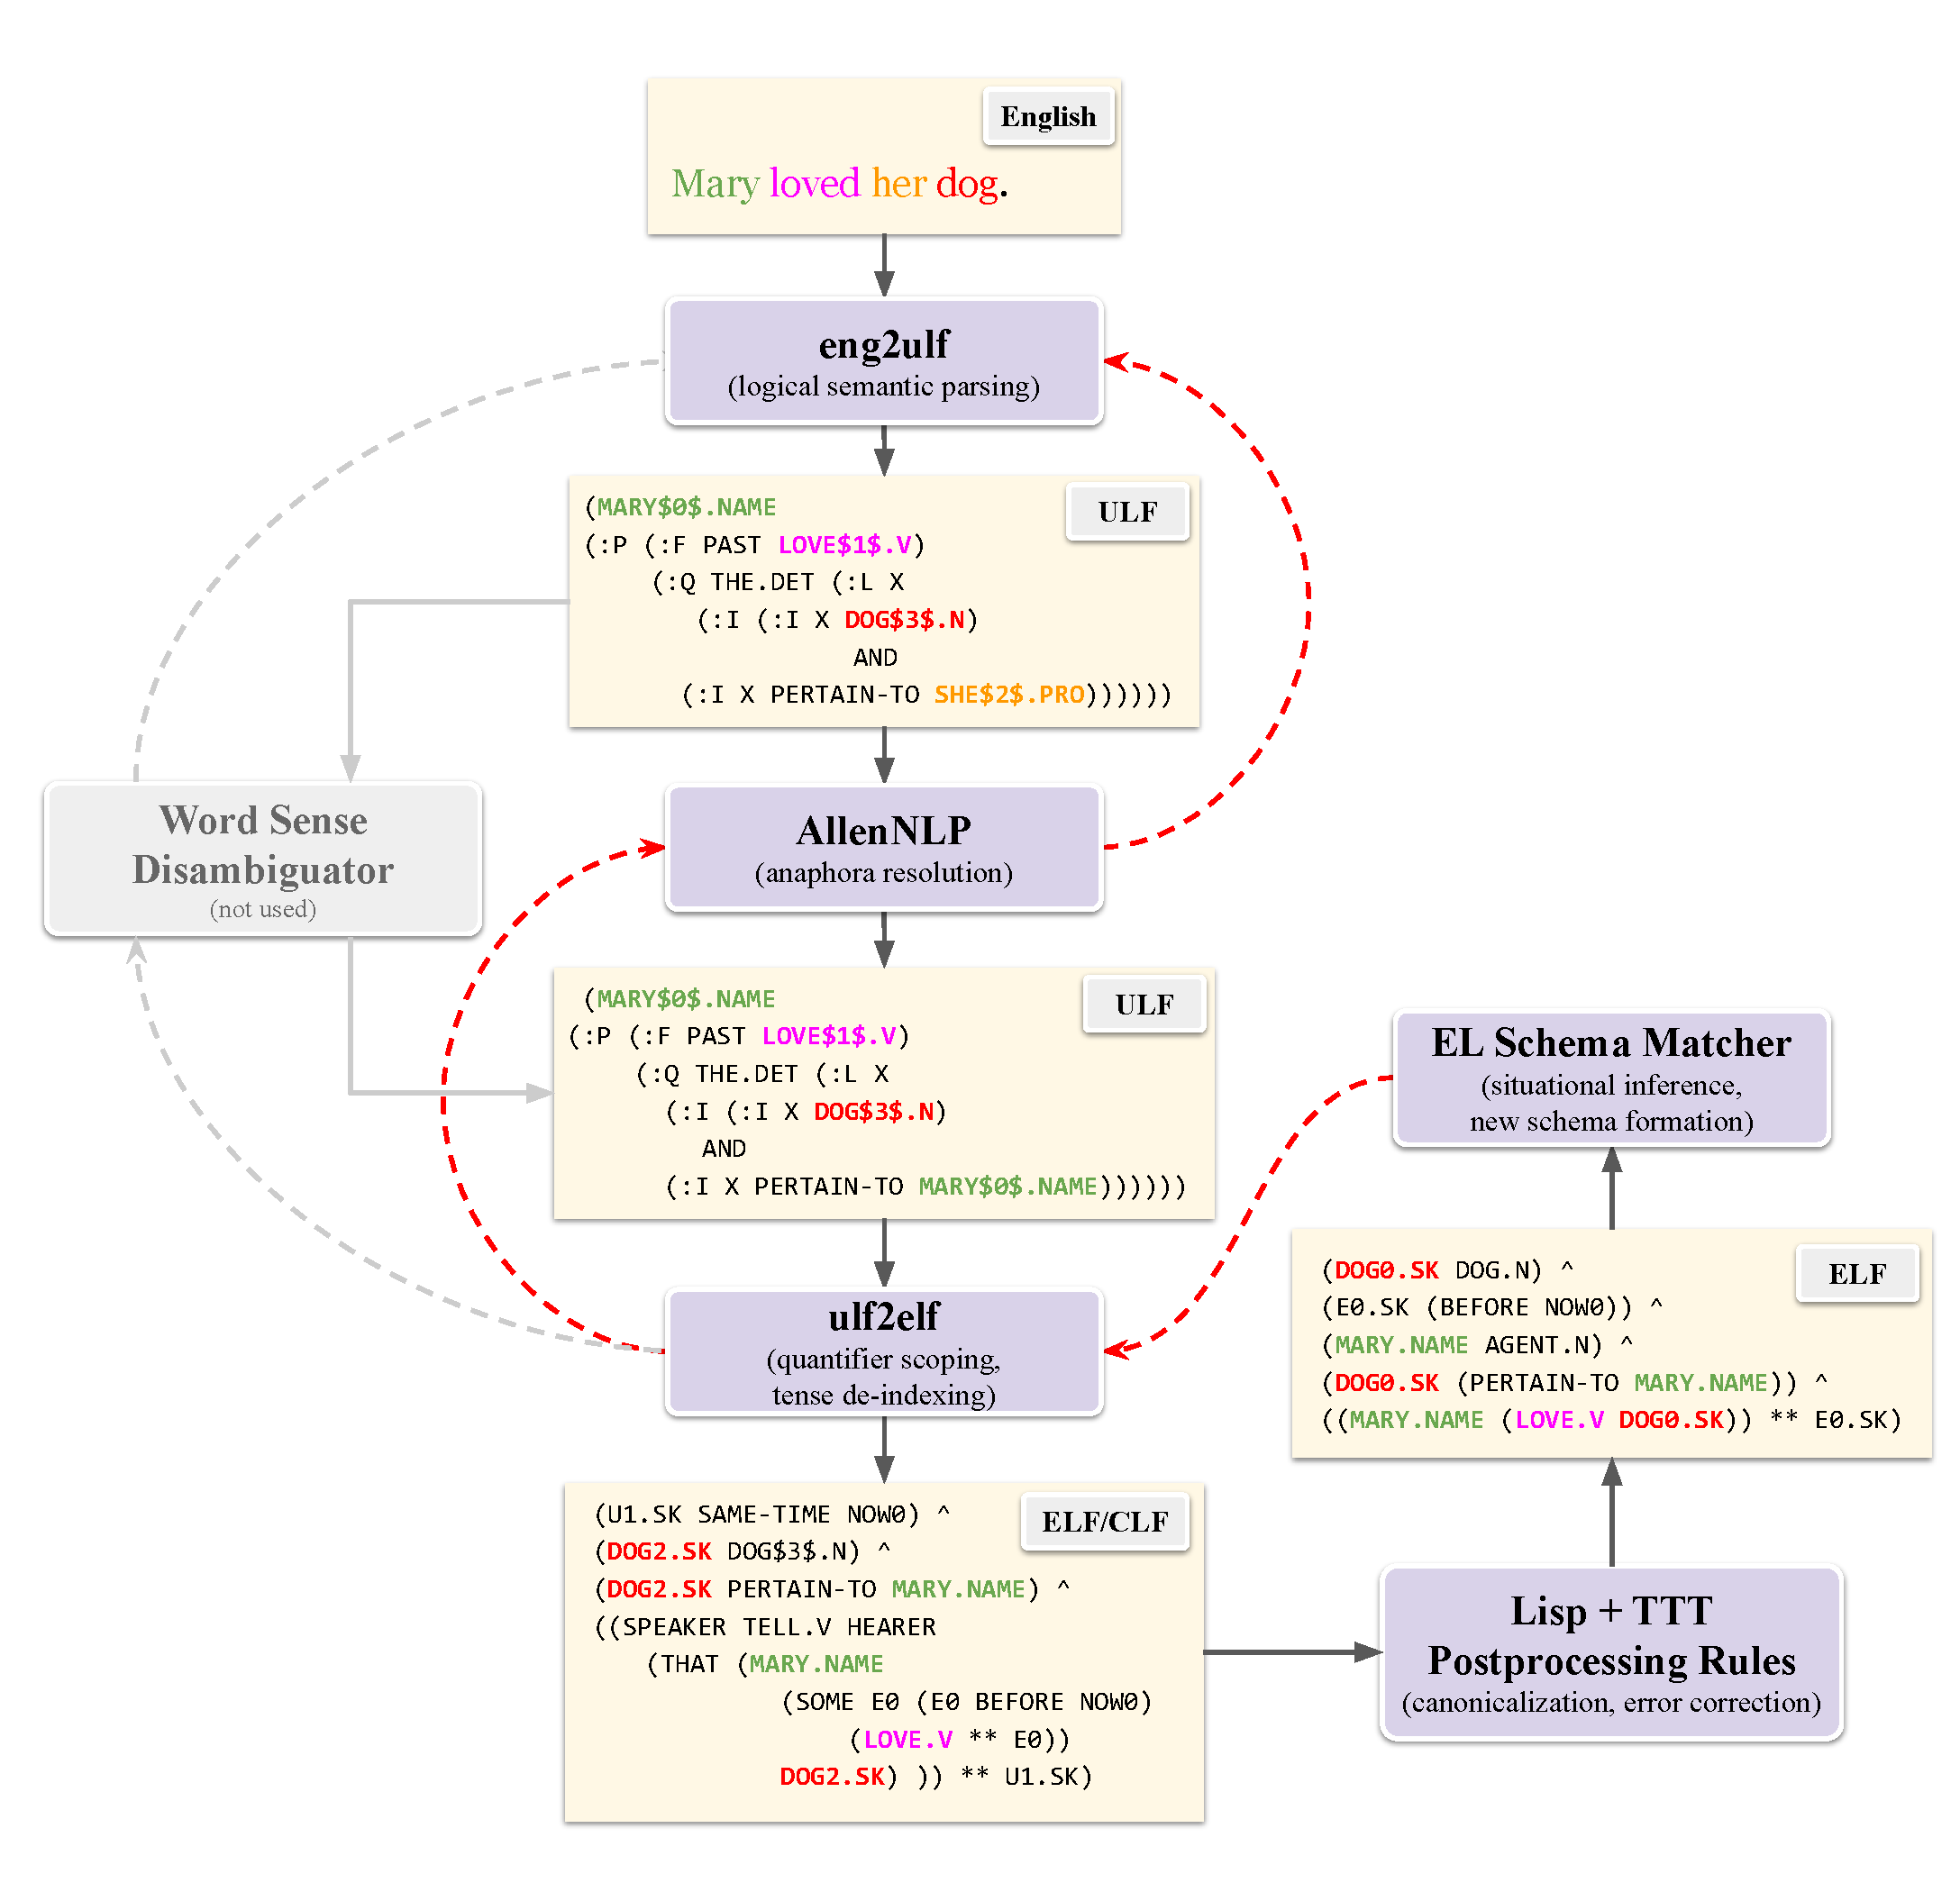
\includegraphics[width=\columnwidth]{CH2_el/parserstages}
    \caption{The information flow diagram of the schema project's EL parser. Rounded, purple rectangles represent software components in the parser pipeline. Sharp, pale rectangles represent the data flowing between components, and are annotated with a specific example of each stage of the parse. Solid, dark arrows represent the forward flow of information between components. Dashed, red arrows represent \textit{theoretical} backward flow of information, i.e., downstream decisions that may prompt changes in upstream decisions; currently, no backward information flow is implemented in our EL parser.}
    \label{fig:my_label}
\end{figure}

\subsection{Evaluating ELF Parser Correctness}
Given a hand-annotated set of English/ELF pairs, we could evaluate the correctness of a parser using some distance metric between a parsed ELF and a ``gold'' ELF. Absent this dataset, however, we adopt an inductive definition of ELF correctness based on a similar definition of ULF correctness and several other measures of correctness for the remaining pipeline steps. The components of a parsed ELF's correctness are as follows:

\begin{enumerate}
    \item The correctness of the parsed ULF.
    \item The accuracy of the word sense disambiguation step, which we take to be $0\%$, as we chose to consider this problem out-of-scope for the current phase of the EL schema project.
    \item The accuracy of the anaphora/coreference resolution step, for which we adopt the accuracy measurements of the underlying coreference analysis engine integrated into the EL parsing pipeline.
    \item The accuracy of quantifier scoping.
    \item The accuracy of canonicalization, which we conservatively define to be the proportion, evaluated on a set of held-out stories, of final ELFs that conform to the grammar given by Figure~\ref{fig:el_cfg}.
    \item Event de-indexing accuracy, which
\end{enumerate}

\begin{figure}
    \centering
    \newcolumntype{L}{>{$}l<{$}}
\newcolumntype{R}{>{$}r<{$}}

\newcommand\LP{\texttt{(}}
\newcommand\RP{\texttt{)}}
\newcommand\SP{\hspace{0.2mm}}
\newcommand\AZ{\texttt{[A-Z]}}

\small
\begin{tabular}{|L|}
\hline\\
{\setlength\tabcolsep{8pt}
\begin{tabular}{L R L}
%\begin{longtable}{L R L}
\phi &\Coloneqq &\phi_{atom}\\
&| &\texttt{(not}~\phi\texttt{)}\\
&| &\texttt{(or}~\phi^{+}\texttt{)}\\
&| &\texttt{(and}~\phi^{+}\texttt{)}\\
&| &\texttt{(if}~\phi~\hspace{0.2mm}~\phi~\texttt{)}\\
&&\\
\phi_{atom} &\Coloneqq &\texttt{(}~I~\hspace{0.2mm}~P~\texttt{)}\\
&| &\texttt{(}\phi~\texttt{**}~I\texttt{)}\\
&| &\LP~M~\SP~\phi~\RP\\
&| &\LP~I~\SP~P~\SP~I^{+}~\RP\\
&&\\
I_{lex} &\Coloneqq &[0-9]^{*}\\
&| &\texttt{[A-Z]}^{*}.\texttt{SK}\\
&| &\texttt{[A-Z]}^{*}.\texttt{PRO}\\
&| &\texttt{[A-Z]}^{*}.\texttt{NAME}\\
&| &?\texttt{[A-Z]}\\
&&\\
I &\Coloneqq &I_{lex}\\
&| &\LP~\texttt{K}~\SP~P~\RP\\
&| &\LP~\texttt{KA}~\SP~P~\RP\\
&| &\LP~\texttt{KE}~\SP~\phi~\RP\\
&| &\LP~\texttt{THAT}~\SP~\phi~\RP\\
&| &\LP~\AZ.\texttt{F}~\SP~I^{+}~\RP\\
&| &\LP~\texttt{[A-Z].DET}~\SP~P~\RP\\
&| &\LP~\texttt{SET-OF}~\SP~I^{+}~\RP\\
%\end{longtable}}
\end{tabular}}
{\setlength\tabcolsep{8pt}
\begin{tabular}{L R L}
%\begin{longtable}{L R L}
P_{atom} &\Coloneqq &\AZ.\texttt{N}\\
&| &\AZ.\texttt{V}\\
&| &\AZ.\texttt{A}\\
&| &\AZ.\texttt{P}\\
&| &\LP~\lambda~\SP~\LP~\AZ~^{*}~\RP~\SP~\phi~\RP\\
&| &\LP~\texttt{PASV}~\SP~\AZ.\texttt{V}~\RP\\
&&\\
P &\Coloneqq &P_{atom}\\
&| &\LP~P~\SP~I^{+}~\RP\\
&| &\LP~M~\SP~P~\RP\\
&&\\
M &\Coloneqq &\AZ.\texttt{ADV-[AEFS]}\\
&| &\LP~\texttt{ADV-[AEFS]}~\SP~P~\RP\\
&| &\LP~\texttt{ADV-[AEFS]}~\SP~M~\RP\\
&| &\texttt{PLUR}\\
\end{tabular}}\\
\vspace{0.2mm}\\
\hline
\end{tabular}
%\end{longtable}}
    \normalsize
    \caption{A context-free grammar representing the simplified Episodic Logic language used for EL schemas. $\phi$ and $\phi_{atom}$ are the rules for forming composite and atomic propositions, respectively; $P$ and $P_{atom}$ are similar rules for complex and atomic predicates. $M$ is a rule for forming predicate modifiers, and $I$ is a rule for forming domain individuals in the EL ontology. The atomic individual rule, $I_{lex}$, may form names, pronouns, Skolem constants, numbers, and variables.}
    \label{fig:el_cfg}
\end{figure}

\subsection{ULF-to-ELF Conversion}
In converting ULFs to ELFs, we adapt the implementation of the EL parser given by \citet{schubert-2014-treebank} to accept pre-formed ULFs rather than creating its own from Treebank parses. Having separated ULF into a prior pipeline step, we refer to this modified parser as \texttt{ulf2elf}. \texttt{ulf2elf} handles quantifier scoping, tense de-indexing, and some canonicalization steps.
%We discuss those steps here.

%\subsubsection{Utilizing Syntactic Information}
%ULF's proximity to the linguistic form of English imbues it with syntactically-derived information that may be absent in the final, more abstract EL form.
Although canonicalization and post-processing of the ELFs, detailed in \ref{subsec:postproc}, are typically performed after arriving at ELFs, some transductions must be performed, or noted down for later performance, at an earlier stage in the pipeline with access to this syntactic information in the ULFs.
%For example, the predicate-argument structure of the sentence \textit{``Kim used to sleep.''}, and its corresponding ULF \texttt{(KIM.NAME ((PAST USE.V) (KA SLEEP.V)))}, centers around the root verb predicate, \el{USE.V}, which is parsed into past tense and assigned the reified kind-of-action argument \el{(KA SLEEP.V)}.
%The de-indexing algorithm used to decode explicit event times from grammatical tense will transmute this syntactic form into the final ELFs \texttt{\texttt{(E1.SK BEFORE NOW1)} and \texttt{((KIM.NAME (USE.V (KA SLEEP.V))) ** E1.SK)}}.
%Recovery of the original syntax is difficult from this ELF: its source sentence might have been \textit{``Kim used to sleep.''}, but might also have been \textit{``Kim was using [the action of sleeping].''}, whose past progressive tense implies a totally different semantics.
%Therefore, we normalize the \textit{used to} form during the ULF stage, converting it 
%Another example is the effect of pronoun choice on quantifier scoping.
%During ULF-to-ELF conversion, possessive pronoun determiners, e.g. \texttt{(HER.D TOY.N)}, are transmuted into lambda predicates under the scope of the pronoun's referent, e.g. \texttt{(THE.D (L X ((X TOY.N) AND (X PERTAIN-TO \textbf{Y}))))}, where the referent, \texttt{\textbf{Y}} is resolved later.
%Because the scope of Y is not known---it could be universally quantified, as in \textit{``Every girl loves her toy.''}---


\subsubsection{Quantifier Scoping}

\subsubsection{Tense De-Indexing}

\subsection{Anaphora Resolution}

\subsection{Word Sense Disambiguation}

\subsection{Post-processing}
\label{subsec:postproc}
The final ELFs obtained from the existing ULF-to-ELF transduction implementation by \citet{schubert-2014-treebank} (heretofore referred to as \texttt{ulf2elf}) are not immediately suitable for use in the schema system; the complex, nested formulas that \texttt{ulf2elf} outputs often require further breakdown and Skolemization to align with the simple, canonicalized formulas found in EL schemas. The simplified EL grammar we assume within the schema system is given by Figure~\ref{fig:el_cfg}; this grammar defines what a ``correct'' EL formula is in the context EL schemas. Even without assuming such a restrictive grammar, however, \texttt{ulf2elf} still introduces a significant number of errors into its output ELFs. Fortunately, however, as \texttt{ulf2elf} is a deterministic, rule-based program, many error types can be classified into patterns and fixed with additional post-processing rules, which we describe here.

We post-process \texttt{ulf2elf} output formulas by iteratively applying two sets of rules---one set written in Lisp and the other implemented as a set of TTT transductions---until a full iteration passes with no changes made. Though more computationally expensive, the Lisp post-processing rules allow for more complicated fixes than TTT would. All of the rules, regardless of implementation, fall into one of the following four categories:

% TODO: rewrite the following subsubs; they're pasted from an email I wrote to Len
\subsubsection{Canonicalization Rules}
These rules perform top-level Skolemization, conjunction splitting, lambda-predicate splitting and removal, normalization of parentheses, re-arrangement of sentential operators and modifiers, and other similar transductions meant to reduce the size and standardize the form of complex ELFs. These rules were developed with the theory and literature of EL in mind, and were not crafted to improve performance on a development story corpus.

\subsubsection{Error Correction Rules}
Rules that fix strange artifacts of the imperfect parsing, whether ULF or ELF parsing, up to that point; some formulas just come out in invalid ways but in identifiable patterns, so rules can be written for them. These were developed on a dev set of stories and evaluated on a test set of stories to see how many invalid ELFs were made valid. They're highly technical and granular.

\subsubsection{Simplifying Rules}
Rules that convert formulas into equivalent and/or more meaningful ones, like "There~is~X"~$\Rightarrow$~"X~is", or, in the case of a less equivalent but more useful transduction, the removal of progressive markers from verbs to make sure they play nicer with the simple event schemas. Some of these rules, like the progressive removal rule, have semantic compromises in order to minimize the already massive engineering effort required to get ELFs to match between schemas and stories. These were developed on a dev set of stories.

\subsubsection{Schema-Specific Rules}
Rules that do things that are just nice for schema learning. One example is adding (X AGENT.N) to stories where X is a lexical name or personal pronoun. Another example is shifting past-tense stories forward in time to "NOW", because past-tense stories only have (BEFORE NOW\#) as their deindexing relations, which ends up not imposing any ordering constraints between the story episodes; I convert these to AT-ABOUT, effectively making the story present-tense, to get that ordering. These were developed without reference to any specific story corpus, and mostly just occurred to me as I was programming.

\iffalse
This section describes the means by which we parse Episodic Logical Forms (ELFs) from English sentences. When constructing the parser, we opted not to construct an explicit dataset of ELF/English pairs, as is customary in many semantic parsing endeavors. Instead, we exploit the structure of the EL parsing pipeline (Figure~\ref{fig:el_pipeline}), in which most semantic parsing is handled by the ULF parser. Because a hand-annotated ULF/English dataset \citep{kim2019IWCS} and several ULF parsers \citep{kim2021transition,kim2021naloma} already exist, we can implement only those remaining steps necessary to obtain the final ELFs.

In Section~\ref{subsec:ulf}, we describe and compare existing ULF parsers, including a novel language model-based parser developed as part of the schema project. Then, in Section~\ref{subsec:elparsing}, we discuss the processing steps necessary to obtain ELFs from ULFs.
\fi